\documentclass[14pt,aspectratio=169]{beamer}
\usetheme{Marburg}
\graphicspath{{Arquivos/}}
\usepackage[utf8]{inputenc}
\usepackage[english]{babel}
\usepackage[T1]{fontenc}
\usepackage{amsmath}
\usepackage{amsfonts}
\usepackage{amssymb}
\usepackage{graphicx}
\usepackage{bibentry}

\definecolor{mygreen}{rgb}{0,0.6,0}
\definecolor{mygray}{rgb}{0.5,0.5,0.5}
\definecolor{mymauve}{rgb}{0.58,0,0.82}
\usepackage{listings}
\lstset{ 
  backgroundcolor=\color{white},   % choose the background color; you must add \usepackage{color} or \usepackage{xcolor}; should come as last argument
  basicstyle=\scriptsize\ttfamily,        % the size of the fonts that are used for the code
  breakatwhitespace=false,         % sets if automatic breaks should only happen at whitespace
  breaklines=true,                 % sets automatic line breaking
  captionpos=b,                    % sets the caption-position to bottom
  commentstyle=\color{mygreen},    % comment style
  deletekeywords={...},            % if you want to delete keywords from the given language
  escapeinside={\%*}{*)},          % if you want to add LaTeX within your code
  extendedchars=true,              % lets you use non-ASCII characters; for 8-bits encodings only, does not work with UTF-8
  firstnumber=1,                % start line enumeration with line 1000
  frame=single,	                   % adds a frame around the code
  keepspaces=true,                 % keeps spaces in text, useful for keeping indentation of code (possibly needs columns=flexible)
  keywordstyle=\color{blue},       % keyword style
  language=Python,                 % the language of the code
  morekeywords={*,...},            % if you want to add more keywords to the set
  numbers=left,                    % where to put the line-numbers; possible values are (none, left, right)
  numbersep=5pt,                   % how far the line-numbers are from the code
  numberstyle=\tiny\color{mygray}, % the style that is used for the line-numbers
  rulecolor=\color{black},         % if not set, the frame-color may be changed on line-breaks within not-black text (e.g. comments (green here))
  showspaces=false,                % show spaces everywhere adding particular underscores; it overrides 'showstringspaces'
  showstringspaces=false,          % underline spaces within strings only
  showtabs=false,                  % show tabs within strings adding particular underscores
  stepnumber=2,                    % the step between two line-numbers. If it's 1, each line will be numbered
  stringstyle=\color{mymauve},     % string literal style
  tabsize=2,	                   % sets default tabsize to 2 spaces
  title=\lstname                   % show the filename of files included with \lstinputlisting; also try caption instead of title
}
\author{Katarina Popović, Dušan Pantelić, Dejan Bokić, Nikola Stojević}
\newcommand{\TT}{Podrška objektno orijentisanom programiranju u jezicima C++, Objective C, Java, C\#, Ada i Ruby}
\newcommand{\TB}{Texto Bíblico}
\newcommand{\DT}{Deuteronômio 26.1-15}

\title{Podrška objektno orijentisanom programiranju u jezicima C++, Objective C, Java, C\#, Ada i Ruby}
%\setbeamercovered{transparent} 
\institute{\small{Seminarski rad u okviru kursa\\Metodologija stručnog i naučnog rada\\ Matematički fakultet}}
\date{Maj 2019} 
%\subject{} 
\begin{document}

\begin{frame}
\titlepage
\end{frame}

\begin{frame}{Sadržaj}
	\tableofcontents
\end{frame}

\section{Uvod}
\begin{frame}[fragile]{Uvod}
\begin{itemize}
\item Programska paradigma
\item Princip jedinstvene odgovornosti
\item Enkapsulacija
\item Nasleđivanje
\item Polimorfizam
\item Apstrakcija
\end{itemize}
\end{frame}

\section{C++}
\begin{frame}[fragile]{C++}
\begin{itemize}
\item C++ je delimično objektno orijentisan jezik
	\begin{itemize}
		\item Main funkcija izvan klase
		\item Koncept globalne promenljive
		\item Postojanje friend funkcija
	\end{itemize}
\item Enkapsulacija u C++
	\begin{itemize}
		\item public, protected i private sekcije
	\end{itemize}
\item Nasleđivanje u C++
	\begin{itemize}
		\item public, protected i private nasleđivanje
		\item virtuelno nasleđivanje
	\end{itemize}
\item Polimorfizam u C++
	\begin{itemize}
		\item polimorfizam u vreme kompilacije
		\item polimorfizam u vreme izvršavanja
	\end{itemize}
\item Apstrakcija u C++
\end{itemize}
\end{frame}


\section{Objetive C}
\begin{frame}[fragile]{Objetive C}
\begin{itemize}
\item Definisanje klasa u dve sekcije:
	\begin{itemize}
		\item {\em\textbf{@interface}}, za deklaraciju
		\item {\em\textbf{@implementation}}, za implementaciju
	\end{itemize}
\item Enkapsulacija
	\begin{itemize}
		\item Atributi su podrazumevano privatni
		\item Navođenje atributa u podsekcijama {\em\textbf{@property}} i {\em\textbf{@synthesize}}, generišu se metode javnog pristupa
	\end{itemize}
\item Nasleđivanje ( označava simbolom ':' )
\item Polimorfizam
	\begin{itemize}
		\item U vreme kompilacije, nije omogućeno
		\item U vreme izvršavanja
	\end{itemize}
\item Apstrakcija
	\begin{itemize}
		\item Nema koncepta apstraktnih klasa
		\item Protokoli označavaju interfejse ({\em\textbf{@protocol, @required, @optional}})
	\end{itemize}
\end{itemize}
\end{frame}

\begin{frame}[fragile]{Objective C}
\begin{lstlisting}[caption={Primer koda u Objective C jeziku},frame=single, label=ObjectiveC]
@interface Employee : NSObject {
   double salary;	@public int age;}
@property(nonatomic, readwrite) double salary; 
- (void)display;
@end # `-' za metode instance, `+' za klasne metode(static)
@implementation Employee
@synthesize salary; 
- (void)display { NSLog(@"Employee salary is %f", salary); }
@end # (id) tip koji je kompaktibilan svakom objektu
@interface Driver : Employee { NSString* truck; }
- (id)initWithTruck:(NSString*)model;
@end # self oznacava tekuci objekat
@implementation Driver
- (id)initWithTruck:(NSString*)model {
   truck = model;	return self;  }
- (void)display { NSLog(@"Driver salary is %f", salary); } @end
int main(int argc, const char * argv[]) {
   NSAutoreleasePool * pool = [[NSAutoreleasePool alloc] init];
   Employee *empl = [[Driver alloc]initWithTruck:@"Mercedes"];
   empl.salary = 5.0;  empl->age = 33;
   [empl display];
   [pool drain];
   return 0;
}}
\end{lstlisting}
\end{frame}

\section{Java}
\begin{frame}[fragile]{Java}
\begin{itemize}
\item Klase definisanje ({\em\textbf{class}})
	\begin{itemize}
		\item  instanciranje  ({\em \textbf{new}}) konstruktorima
	\end{itemize}
\item Enkapsulacija
\begin{table}
	\scalebox{0.8}{
	\begin{tabular}{|l|c|c|c|c|} \hline
	Modifikator &Klasa &Paket &Podklasa &Svet\\ \hline
	public &Da &Da &Da &Da\\ \hline
	protected &Da &Da &Da &Ne\\ \hline
	podrazumevani &Da &Da &Ne &Ne\\ \hline
	private &Da &Ne &Ne &Ne\\ \hline
	\end{tabular}}
	\begin{itemize}
		\item  Metode javnog pristupa (eng. {\em getters and setters})
	\end{itemize}
\end{table}
\item Polimorfizam
	\begin{enumerate}
		\item U vreme kompilacije, preopterećenost (eng. {\em overloading})
		\item U vreme izvršavanja, preklapanje (eng. {\em overriding})
	\end{enumerate}	
\end{itemize}	
\end{frame}

\begin{frame}[fragile]
\begin{itemize}

\item Nasleđivanje ({\em\textbf{extends}})
	\begin{figure}[h!]
	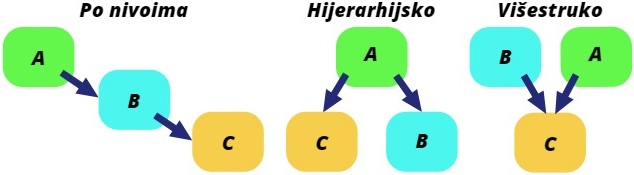
\includegraphics[scale=0.7]{slike/nasledjivanje.jpg}
	\end{figure}	
\item Apstrakcija
	\begin{enumerate}
		\item Apstraktne klase ({\em \textbf{abstract}} )
		\item Interfejs ({\em \textbf{interface, implements}} )
		\begin{itemize}
			\item Klasa može implementirati više interfejsa, dok može nasleđivati samo jednu klasu
		\end{itemize}
	\end{enumerate}	
\end{itemize}
\end{frame}

\section{C\#}
\begin{frame}[fragile]{C\#}
\begin{itemize}
\item C\# 
	\begin{itemize}
		\item C\# je jednostavan, moderan, objektno-orijentisan jezik
		\item Nudi punu podršku objektno orijentisanom programiranju
		\item Ne podržava druge paradigme ali koristi svoje imperativne strukture
	\end{itemize}
\item Enkapsulacija u C\#
	\begin{itemize}
		\item public, private, protected, internal i protected internal sekcije
	\end{itemize}
\item Nasleđivanje u C\#
	\begin{itemize}
		\item može da bude direktno ili indirektno
		\item samo jednostruko nasleđivanje je podržano
	\end{itemize}
\item Polimorfizam u C\#
	\begin{itemize}
		\item polimorfizam vremena kompiliranja
		\item polimorfizam vremena izvođenja
	\end{itemize}
\item Apstrakcija u C\#
         \begin{itemize} 
		\item Apstraktni tip se konstruiše dodavanjem abstract u deklaraciji
	\end{itemize}
\end{itemize}
\end{frame}

\section{Ada}
\begin{frame}[fragile]{Ada}
\begin{itemize}
	\item Ada ne sledi model klase zasnovan na jednom konstruktoru
	\begin{itemize}
		\item Odvojene karakteristike tipova unutar paketa
		\item Moguće postojanje funkcija i procedura u paketu
	\end{itemize}
	\item Enkapsulacija
	\begin{itemize}
		\item Privatnost se određuje na nivou paketa
		\item private, limited private
	\end{itemize}
	\item Nasleđivanje
	\begin{itemize}
		\item Implementirano nasleđivanje po nivoima i hijerarhijsko
		\item Višestruko nasleđivanje je moguće implementirati 
	\end{itemize}
	\item Polimorfizam
	\begin{itemize}
		\item Pomoću nasleđivanja, apstrkatnih tipova i podtipova
	\end{itemize}
	\item Apstrakcija
	\begin{itemize}
		\item Apstraktni tip se konstruiše dodavanjem abstract u deklaraciji
	\end{itemize}
\end{itemize}
\end{frame}

\begin{frame}[fragile]{Ada \small{- primer koda}}
\begin{lstlisting}[frame=single, label=lst:adaDeklaracija]
package Employees is 
	type Employee is tagged 
	record
		Name: String;
	end record;
	procedure Set_Name(Obj: in out Employee; Name: String);
	function Print(E: Employee) return String;
end Employees;

package Drivers
	type Driver is new Employees.Employee with record
		Driver_ID: Integer;
	end record;
	procedure Set_D(Obj: in out Employee; Name: String);
	overriding function Print(D: Driver) return String;
end Drivers;
\end{lstlisting}
\end{frame}

\section{Ruby}
\begin{frame}[fragile]{Ruby}
\begin{itemize}
	\item Kreiranje klasa u jeziku Ruby
	\begin{itemize}
		\item Standardni metod initialize, ponaša se kao konstruktor
	\end{itemize}
	\item Enkapsulacija
	\begin{itemize}
		\item public, protected i private
		\item attr\_accessor(čitanje i izmena), attr\_reader(čitanje) i attr\_writer(izmena)
	\end{itemize}
	\item Nasleđivanje
	\begin{itemize}
		\item Implementirano nasleđivanje po nivoima i hijerarhijsko
		\item Višestruko nasleđivanje nije podržano
	\end{itemize}
	\item Polimorfizam
	\begin{itemize}
		\item Pomoću nasleđivanja
		\item Duck typing
	\end{itemize}
	\item Apstrakcija
	\begin{itemize}
		\item Nema direktnu podršku
		\item Moguće implementiranje sličnog ponašanja pomoću nasleđivanja
	\end{itemize}
\end{itemize}
\end{frame}

\begin{frame}[fragile]{Ruby \small{- primer koda}}
\begin{lstlisting}[frame=single, label=lst:rubyDeklaracija]
class Employee
	attr_accessor :name
	def initialize(name)
		@name = name
		print()
	end
	def print
		puts "Employee: #{@name}."
	end
end

class Driver < Employee
	def initialize(name)
		@name = name
		print()
	end
	private
	def print
		puts "Driver: #{@name}."
	end
end

emp = Employee.new("John")
drv = Driver.new("John")
\end{lstlisting}
\end{frame}

\section{Literatura}
\begin{frame}[fragile]{Literatura}
\begin{itemize}
	\scriptsize
	\item Introduction to Ada. on-line at: \url{https://learn.adacore.com/courses/intro-to-ada/index.html}
	\item Object C apple documentation. on-line at: \url{https://developer.apple.com/library/archive/documentation/Cocoa/Conceptual/ObjectiveC}
	\item Ruby - Object Oriented. on-line at: \url{https://www.tutorialspoint.com/ruby/ruby_object_oriented.htm}
	\item Gary Bennet, Brad Lees and MItchell Fisher. Objective-C for Absolute Beginners: IPhone, iPad and Mac Programming Made Easy. Apress, Berkely, CA, USA, 3rd edition, 2016
	\item AdaCore experts. High-Integrity Object-Oriented Programming in Ada. AdaCore(www.adacore.com), 1.2 release edition, 2011. on-line at: \url{http://extranet.eu.adacore.com/articles/HighIntegrityAda.pdf}
	\item Hal Fulton. The Ruby Way. Sams Publishing, 2001.
	\item Cay S Horstmann. Core Java SE 9 for the Impatient. Addison-Wesley Professional, 2017.
	\item Aayushi Johari. Object Oriented Programming - Java OOPs Concepts With Examples, 2018. on-line at: \url{https://www.edureka.co/blog/object-oriented-programming/}
	\item Stephen Prata. C++ Primer Plus (5th Edition) (Primer Plus (Sams)). Sams, Indianapolis, IN, USA, 2004
\end{itemize}
\bibliographystyle{unsrt}
\end{frame}


\end{document}